%!TEX root = ../main.tex

\chapter{How to write thesis in LaTeX\label{chap:how_to}}

\section{Mathematical notation with LaTeX}

\section{Abbreviations with Acronym}

Abbreviations are handled by the \emph{acronym} package.
Example sentence with abbreviations: ``\ac{UAV} is a flying vehicle that commonly uses \ac{LiDAR} and \ac{GPS} receiver''.
Please, read the documentation (\url{http://mirrors.ctan.org/macros/latex/contrib/acronym/acronym.pdf}).

\section{Units of measurements with Siunitx}

Typesetting units has never been easier with the Siunitx package.
Acceleration is measure in \si{\meter\per\second\squared}.
Gravity accelerates objects at a rate $\approx \SI{9.81}{\meter\per\second\squared}$ near the sea level.
You can define your own units if you want.

\section{2D Diagrams with Tikz}

\section{Data plots with PGFPlots}

\begin{itemize}
  \item Documentation and manual: \url{https://ctan.org/pkg/pgfplots}
  \item Compile the plots individually and then include the pdfs, because it can take a long time.
  \item Example located in \texttt{fig/plots/example\_plot}, see \reffig{fig:pgfplots}.
  \item You could include the latex file directly, however, it will take longer time to compile and platforms such as Overleaf can have a problem with that.
\end{itemize}

\begin{figure}[!h]
  \centering
  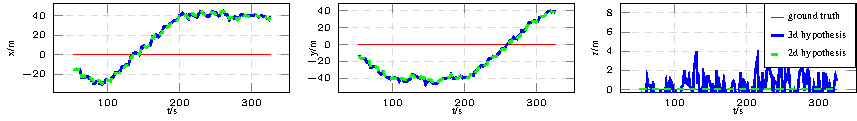
\includegraphics[width=1.0\textwidth]{./fig/plots/example_plot/hypotheses.pdf}
  \caption{Example of a 2D plot using \emph{PGFPlots}.}
  \label{fig:pgfplots}
\end{figure}

\section{3D Plots with Sketch}

See the example in \reffig{fig:coordinate_systems}.

\begin{itemize}
  \item Documentation and manual: \url{http://www.frontiernet.net/~eugene.ressler/}
  \item Cross-compilation from \emph{Sketch} to \emph{pdf} using the \texttt{fig/sketch/compile\_sketch.sh} script.
\end{itemize}

\begin{figure}[!h]
  \centering
  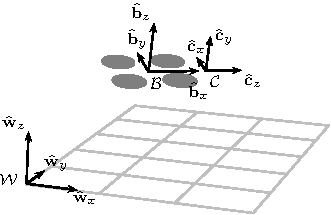
\includegraphics[width=0.4\textwidth]{./fig/sketch/coordinate_frames.pdf}
  \caption{Depiction of the used coordinate systems. The image was drawn using \emph{Sketch}.}
  \label{fig:coordinate_systems}
\end{figure}

\section{Image collages with Subfig}

\section{Citations with Biblatex}

\section{Image overlays with Tikz}
